\section{RESULTS AND DISCUSSION}

\noindent\fbox{\parbox{0.95\linewidth}{\singlespacing\small\textbf{DRAFT.} This chapter is a draft for review.}}

All results are comparisons between simulated strategies under the baseline assumptions of Table~\ref{table:params}. They are not field predictions. Two configurations are read as different only when the ratio of their means exceeds the pooled noise band (see Replicates and the reading of differences in the Methodology).

\subsection{Strategy Comparison}

Table~\ref{table:results} gives the main comparison. On window A, no control gave 10.8 million K-days of cumulative pest load, with 96.5\% of cane cells ever infested. Every control strategy cut the load by at least 82\%. Chemical control without efficacy decline gave the lowest load, 0.69 times the pooled biological and hybrid mean of 43,258 K-days (14 runs). Biological and hybrid control were indistinguishable. At baseline the hybrid applied no chemical, because treating at Level 1 every 14 days kept every farm below Level 3, and its pooled mean was 1.02 times the biological mean. Chemical control with efficacy halving every 20 and every 10 applications per farm gave 17.4 and 44.4 times the biological and hybrid pool.

The island runs gave the same order. Their loads are not comparable with window A in size, because the island seed is spread over 11 units and the island holds about 11 times as much cane. Without control, 64\% of the island's cane cells were ever infested by the end of the run, against 2.7\% to 8.2\% under the control strategies.

Biological control used more applications than chemical control without decline: 54,588 against 34,882 on window A, and 71,334 against 48,560 on the island. This follows from the model rules: the fungus kills 0.9 times as much per application, so more farms reach the trigger again. Declining chemical efficacy raised the number of chemical applications, to 85,602 and 125,474 on window A at halving every 20 and every 10 applications.

\begin{table}[!htbp]
\vspace{2ex}
\centering
\small
\caption{Main comparison, 1,095 days after seeding. Load is the mean cumulative pest load in K-days. Ever is the share of cane cells ever infested. Applications are mean farm-level treatment events (chemical for the chemical strategies, fungal for the biological and hybrid strategies; the hybrid applied no chemical). Two runs per configuration, three for island no control. Decline $n$: chemical efficacy halves every $n$ applications per farm.}
\label{table:results}
\begin{tabular}{lrrrrrr}
\hline\hline
 & \multicolumn{3}{c}{Window A} & \multicolumn{3}{c}{Island} \\
Strategy & Load & Ever & Applications & Load & Ever & Applications \\ \hline
Chemical, no decline & 30,013 & 0.19 & 34,882 & 43,950 & 0.027 & 48,560 \\
Hybrid, decline 20 & 42,789 & 0.26 & 53,128 & 63,067 & 0.038 & 73,889 \\
Biological & 44,123 & 0.26 & 54,588 & 60,394 & 0.036 & 71,334 \\
Chemical, decline 20 & 754,011 & 0.34 & 85,602 & 982,778 & 0.051 & 117,911 \\
Chemical, decline 10 & 1,919,710 & 0.49 & 125,474 & 2,539,217 & 0.082 & 178,486 \\
None & 10,763,962 & 0.97 & 0 & 33,213,080 & 0.64 & 0 \\
\hline\hline
\end{tabular}
\end{table}

\subsection{Efficacy Decline}

Figure~\ref{fig:decline} shows chemical control on window A across decline rates. With efficacy halving every 160 or 80 applications per farm, chemical control stayed within or below the biological and hybrid range (0.79 and 0.90 times the pool). At 40 applications it was 3.9 times worse. Chemical control therefore matches biological control only if its efficacy halves no faster than about every 80 applications. This advantage of the fungus follows from the assumption that its efficacy does not decline.

When the fungus also halved every 20 applications, biological control gave 1,205,918 K-days, 1.60 times chemical control at the same rate, and the hybrid gave the lowest load, 0.32 times biological and 0.51 times chemical. At 80 applications, biological control was 1.95 times chemical, and the hybrid tied with biological (ratio 0.89). This is likely because the hybrid counts the two agents' applications separately, so switching agents spreads the decline across them.

\begin{figure}[!htbp]
	\begin{center}
		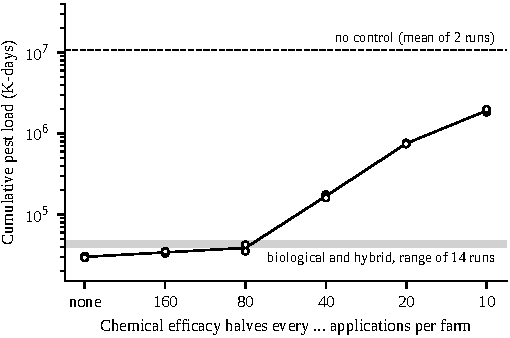
\includegraphics[width=0.7\textwidth]{figures/fig-decline}
		\caption{Chemical control on window A by efficacy-decline rate. Circles are single runs and the line joins means. The band is the range of 14 biological and hybrid runs at baseline. Fungal efficacy does not decline in these runs.}
		\label{fig:decline}
	\end{center}
\end{figure}

\subsection{The Hybrid Strategy}

The hybrid differs from biological control only where farms reach Level 3, and treating at Level 1 every 14 days kept them below it. In the sensitivity screen, the hybrid applied chemicals only where treatment was delayed: a trigger at Level 2 or 3, or re-treatment every 28 days. Rerun with non-declining chemical control, these settings gave a tie when treating only at Level 3 (ratios 0.89 to 1.04), and an ordering of chemical (262,998 K-days), hybrid (693,075), and biological (1,119,909) when re-treating every 28 days. While fungal efficacy holds, the hybrid adds nothing. It helps when both agents lose efficacy quickly.

\subsection{Sensitivity}

The baseline ranking, biological and hybrid tied, then chemical with decline 20, then no control, held in 15 of 18 cases (Table~\ref{table:oat}). No control was last in all 18. When treatment waited for Level 3 or was repeated every 28 days, biological control ranked first. When settlement survival was 0.01, chemical control ranked first, but the outbreak was about 26 times smaller, so this ranking is less certain. The response rules mattered more than any biological parameter: for biological control, waiting for Level 2 raised the load 16.6 times and waiting for Level 3, 33 times. Wind bias, long-jump rate, and the fungus-to-chemical ratio moved loads by less than 1.5 times. Runs with wind from the south-west gave 0.96 to 1.11 times the load of runs with wind from the north-east, inside the noise bands.

\begin{table}[!htbp]
\vspace{2ex}
\centering
\small
\caption{One-at-a-time screen on window A: largest change in load over the four strategies, as the absolute log$_{10}$ ratio to the baseline pool. One run per case. The ranking changed for settlement survival 0.01, a trigger at Level 3, and re-treatment every 28 days.}
\label{table:oat}
\begin{tabular}{lll}
\hline\hline
Assumption & Low, high & Change \\ \hline
Settlement survival & 0.01, 0.10 & 1.96 \\
Trigger level & 2, 3 & 1.81 \\
Re-treatment interval & 7, 28 d & 1.49 \\
Parasitism & 0, 0.668 & 1.16 \\
Neighbour transmission & $\times$0.25, $\times$4 & 0.86 \\
Level thresholds & $\times$0.5, $\times$2 & 0.59 \\
Long-jump probability & 0, 0.2 & 0.17 \\
Fungus-to-chemical ratio & 0.8, 1.0 & 0.17 \\
Wind bias & 0.5, 1.0 & 0.06 \\
\hline\hline
\end{tabular}
\end{table}

\subsection{Hindcast}

Table~\ref{table:hindcast} compares the model with the SRA record. At baseline the model spread too slowly: even without control it reached 0.30 of the validated area. A threefold transmission rate brought no control to 0.98 of it. That rate is one parameter tuned to one number with control ignored, and it was not used in the strategy comparison. The same run fell short earlier in the outbreak: 2,861 ha at the weekly output nearest 11 September 2025, against 4,923 ha recorded for Negros Island on that date \citep{MojicaSevilla2025}. No run matched which municipalities were worst affected (rank correlations of $-0.29$ to 0.22 outside the seeded units). In the hybrid run all infested farms stayed at Level 1, while the provincial survey found 53\%, 31\%, and 16\% of infested farmlots at Levels 1 to 3 \citep{PGNO2026}. Real response is slower and less complete than the model's weekly, error-free trigger: about 53\% of the validated area had been treated by 2 October 2026 \citep{SRA2026FOI}.

\begin{table}[!htbp]
\vspace{2ex}
\centering
\small
\caption{Hindcast, 2 October 2026: model cane area ever infested against the 72,103 ha validated by the SRA \citep{SRA2026FOI}. Hybrid: mean of two runs. Others: one run. $\rho$ is the Spearman correlation with the SRA share by municipality over the 45 unseeded units.}
\label{table:hindcast}
\begin{tabular}{lrrr}
\hline\hline
Run & Area (ha) & Ratio & $\rho$ \\ \hline
Hybrid, baseline & 2,908 & 0.04 & 0.10 \\
None, baseline & 21,275 & 0.30 & $-0.29$ \\
None, long jump 0.2 & 44,072 & 0.61 & 0.22 \\
None, transmission $\times$2.5 & 58,136 & 0.81 & $-0.09$ \\
None, transmission $\times$3 & 70,430 & 0.98 & $-0.18$ \\
None, transmission $\times$4 & 105,535 & 1.46 & $-0.04$ \\
\hline\hline
\end{tabular}
\end{table}

\subsection{Discussion}

Within its assumptions, the model suggests three things. Any control strategy reduces pest load far below no control. Acting early matters more than which agent is used: delaying the trigger or the re-treatment changed loads more than any biological parameter did. The ranking of chemical against biological control turns on two quantities that have not been measured, how fast chemical efficacy declines with repeated use and whether fungal efficacy holds. The biological lead holds only if fungal efficacy holds, and the hybrid is best only when both agents lose efficacy quickly.

The hindcast bounds how far these comparisons can be read. Baseline spread is too slow, the model does not reproduce which municipalities are worst affected, and its farmers respond more promptly than observed. The comparisons are therefore relative, between strategies run under the same assumptions. Data on the repeated-application efficacy of both agents, on spread between fields, and on the timing of real treatment would most change them.
